\newif\ifpaper
%TODO: Uncomment when printing
\papertrue

\ifpaper
	\documentclass[BCOR=3cm,twoside,abstract,a4paper]{scrreprt}
\else
	\documentclass[abstract,a4paper]{scrreprt}
\fi


% Spacing below paragraphs rather than indentations
\usepackage{parskip}

% Fancy Headers and Chapters
\usepackage{fancyhdr}

% Date Formatting
\usepackage[UKenglish]{datetime}

% Images
\usepackage{graphicx}
\graphicspath{{img/}}

% Colours
\usepackage[usenames,dvipsnames]{xcolor}
\definecolor{AberMaroon}{HTML}{952D2E}

% Hyperlinks
\usepackage[colorlinks, urlcolor=AberMaroon, linkcolor=Black, citecolor=AberMaroon]{hyperref}

% Include List of Tables/Figures/Bibliography in Contents
\usepackage[nottoc]{tocbibind}

% Add appendix environment
\usepackage[toc]{appendix}

% Acronyms
\usepackage{acronym}

% Tables
\usepackage{tabularx}
\usepackage{booktabs}
\usepackage{array}
\usepackage{rotating}

% Dingbats for \cmark and \xmark
\usepackage{pifont}
\newcommand{\OK}{\ding{51}}
\newcommand{\KO}{\ding{55}}

% Rotate table headers
\newcommand*\rot{\rotatebox{90}}

% Directory Trees
\usepackage{dirtree}

\usepackage{float}

\usepackage{pdfpages}


\begin{document}

	% Use Roman numerals for preamble pages and hide them
	\pagenumbering{roman}
	\pagestyle{empty}

	\begin{titlepage}
	\begin{center}
	
	~\\
	
	\vspace{3cm}
	\includegraphics[width=0.5\textwidth]{cover/extending_awesome} \\
	\vspace{1.5cm}
	{ \large Final Report for CS39440 Major Project }
	\vspace{1cm}

	\hrule
	\vspace{0.5cm}
	
	\noindent
	\begin{minipage}[t]{0.4\textwidth}
		\begin{flushleft} \large
			\emph{Author:}\\
			Benjamin \textsc{Brooks}\\
			\href{mailto:beb12@aber.ac.uk}{beb12@aber.ac.uk}
		\end{flushleft}
	\end{minipage}%
	\begin{minipage}[t]{0.4\textwidth}
		\begin{flushright} \large
			\emph{Supervisor:} \\
			Dr.~Hannah \textsc{Dee}\\
			\href{mailto:hmd1@aber.ac.uk}{hmd1@aber.ac.uk}
		\end{flushright}
	\end{minipage}
	
	\vspace{0.5cm}
	\hrule

	\vfill

	{\large \today \\ Version 0.1 (Draft)}
	
	\vspace{1cm}
	This report was submitted as partial fulfilment of a BSc degree in Computer Science (inc Integrated Industrial and Professional Training) [G401] \\
	\vspace{1cm}
	\includegraphics[width=0.33\textwidth]{cover/aberystwyth_logo}
	
	% Allow the logo to be closer to the bottom of the page
	\vspace{-2cm}

	\end{center}
\end{titlepage}

	\section*{Declaration of Originality}

In signing below, I confirm that:

\begin{itemize}
	\item This submission is my own work, except where clearly indicated.
	\item I understand that there are severe penalties for plagiarism and other unfair practice, which can lead to loss of marks or even the withholding of a degree.
	\item I have read the sections on unfair practice in the Students' Examinations Hand- book and the relevant sections of the current Student Handbook of the Department of Computer Science.
	\item I understand and agree to abide by the University's regulations governing these issues.
\end{itemize}

\vspace{1cm}

{ \Large
Signature \hrulefill
\hspace{1cm}
Date \hrulefill
}

\section*{Consent to share this work}

In signing below, I hereby agree to this dissertation being made available to other students and academic staff of the Aberystwyth Computer Science Department.

\vspace{1cm}

{ \Large
Signature \hrulefill
\hspace{1cm}
Date \hrulefill
}

\section*{Ethics Form Application Number}

The Ethics Form Application Number for this project is: \textbf{1019}.

\vfill

\begin{center}
	\section*{\center Student Number}
	\includegraphics[width=0.33\textwidth]{beb12-barcode}
\end{center}

\vspace{-3cm}

\ifpaper
	\newpage
	~
\fi

	% Show page number from this point
	\pagestyle{plain}

	\begin{center}
~\\
\vfill

thanks

\vfill
~\\
\end{center}
	\begin{abstract}
	\thispagestyle{plain}
	This is my abstract.
\end{abstract}

	\tableofcontents
	\listoftables
	\listoffigures
	\chapter*{List of Acronyms}
\addcontentsline{toc}{chapter}{List of Acronyms}

% To alphabetise list, use
% sort -fo acronyms-list.tex acronyms-list.tex

\begin{acronym}[XXXXXXXX]
	\acro{ASTRA}{Aberystwyth Student Records and Admissions}
\acro{AU}{Aberystwyth University}
\acro{AWESOME}{The Aberystwyth Web Evaluation Of Module Experiences}
\acro{CI}{Continous Integration}
\acro{i18n}{Internationalisation}
\acro{MEQ}{Module Evaluation Questionnaires}
\acro{MVC}{Model-view-controller}
\acro{OOP}{Object-oriented programming}
\acro{SME}{Student Module Evaluation}
\acro{CSV}{Comma-Separated Values}
\acro{PDO}{PHP Data Objects}
\acro{SQL}{Structured Query Language}
\acro{RDBMS}{Relational Database Management System}

\end{acronym}


	% Use Arabic numerals for main content
	\clearpage
	\pagenumbering{arabic}
	% Use fancy page headings for main content
	\pagestyle{fancy}

	\chapter{Introduction}
\newpage

	\section{Background}
	
	
	
	\section{Analysis}
	
	
	\chapter{Design}
	
	After the security audit, it was apparent that the majority of the codebase needed to be refactored in order to make it object-oriented.
	The decision to rewrite the program was not a light one, by rewriting the program, the scope of extensions to \ac{AWESOME} became much more limited via time constraints.
	
	With the rewrite came the opportunity to utilise both a framework and a design pattern.
	Frameworks were ruled out under the stance that it had to be deployed on a server without shell access.
	However later research discovered that this is achievable in Laravel\footnote{Laravel Homepage: \url{http://laravel.com}}, which would have been the framework of choice for several reasons.
	
	Laravel would have provided a complete, and mature \ac{MVC} framework, as well as an \ac{i18n} framework and a solid basis for \ac{AWESOME}.
	Ultimately, poor research into Laravel on a shell-less server resulted in an attempt to produce a bespoke \ac{MVC} framework, which, unsurprisingly is harder than it first seems.
	
	\section{Programming Language}
	
	The programming language choice was fairly fixed, as it had to be easily runnable on an \ac{AU} server.
	This limited the choice to PHP, but which minor version of PHP was only found out later in the project which is discussed further in \autoref{sec:implementation}.
	
	If this requirement wasn't an issue, Ruby on Rails would have been the ideal candidate for this project, as it already provides an \ac{MVC} framework and gems for \ac{i18n}.
	
	\section{\acl{MVC} Framework}
	
	Since using a framework was ruled out, a custom-made \ac{MVC} framework was written to support this project.
	The design of which is laid out in this section and is very heavily taken from the `Write your own PHP MVC Framework' series of tutorials\cite{php-mvc-tutorial}.
	
	\subsection{Routing}
	
	URL Routing is a way to access specific controllers and views from a URL.
	This works via an Apache rewrite rule, which appends a \$\_GET variable which contains the current requested URL.
	
	\subsection{Directory Structure}
	
	\autoref{fig:mvcdirtree} shows the directory structure of the \ac{MVC} framework. `\textit{src}' is the source code to the program. Inside it contains everything needed to run \ac{AWESOME}.
	Inside `\textit{tests}' are the unit tests to be run automatically by TravisCI and PHPUnit.
	
	`\textit{src/app}' has the MVC classes which are used when the routing engine rewrites URLs.
	`\textit{src/config}' contains the config file for the program.
	In this file, database credentials are set, as well as SMTP mail server settings, some \ac{i18n} settings, and the debug flag which displays errors and shows a feedback form/notice (See \autoref{fig:feedbackform}).
	
	`\textit{src/db}' is a directory for \ac{SQL} dumps for the database schema.
	`\textit{src/i18n}' contains translation files for the \ac{i18n} framework, but more detail is in \autoref{sec:i18nframework}
	
	`\textit{src/lib}' is the `glue' that holds the MVC framework together.
	It contains the autoloader class, the bootstrap script and the third-party, open source PHPMailer\cite{phpmailer} classes used for sending mail via SMTP.
	
	`\textit{src/logs}' is where any PHP errors get logged when debug mode is off. This is in order to hide any potential security issues with displaying errors.
	
	`\textit{src/public}' is the main entry point to the program and where the Apache vhost will be set.
	`\textit{src/public/assets}' contains the Javascript, SASS, CSS, and images used in the HTML.
	Users with a valid token will be taken to their corresponding questionnaire.
	`\textit{src/public/admin}' is protected by HTTP authentication to prevent anybody from creating surveys and sending them out, or reading the results of previous surveys.
	
	\begin{figure}[H]
		\dirtree{%
			.1 AWESOME.
			.2 src.
			.3 app.
			.4 controllers.
			.4 models.
			.4 views.
			.3 config.
			.3 db.
			.3 i18n.
			.3 lib.
			.3 logs.
			.3 public.
			.4 admin.
			.4 assets.
			.2 tests.
		}
		\caption{Directory structure of the \acs{MVC} Framework}
		\label{fig:mvcdirtree}
	\end{figure}	
	
	\section{Internationalisation Framework}
	\label{sec:i18nframework}
	
	The \ac{i18n} framework is a standalone \ac{OOP} module which utilises JSON formatted files with strings for translation.
	
	\section{Database Schema}
	
	The database schema (see \autoref{fig:schema}) used is very similar to the prototype version.
	Documentation needed to be written for the existing schema, so the opportunity was taken to make some changes in the structure of the database before this happened.
	The old database schema did not use any foreign key constraints, nor was the use of primary keys ideal.
	
	Foreign keys are very useful to have in a system like this, as orphaned rows can be cleaned up nicely with a cascade delete.
	This prevents any data remaining in the table incase it is missed by an \ac{SQL} query that hasn't been updated in the code.
	
	I also made some changes to the way things were named, mostly to prevent confusion.
	In the new schema, a survey is a set of questionnaires, each of which is tailored to a specific student.
	In the old schema, everything was called a questionnaire, which led to confusion between a group of questionnaires and a single questionnaire.

	Additional changes need to be made in order for \ac{AWESOME} to support multiple departments across the university, but this is out of the scope of the dissertation, although this feature is on the roadmap if \ac{AWESOME} is to be used university-wide.
	
	\begin{figure}[H]
		\hspace{-0.165\textwidth}
		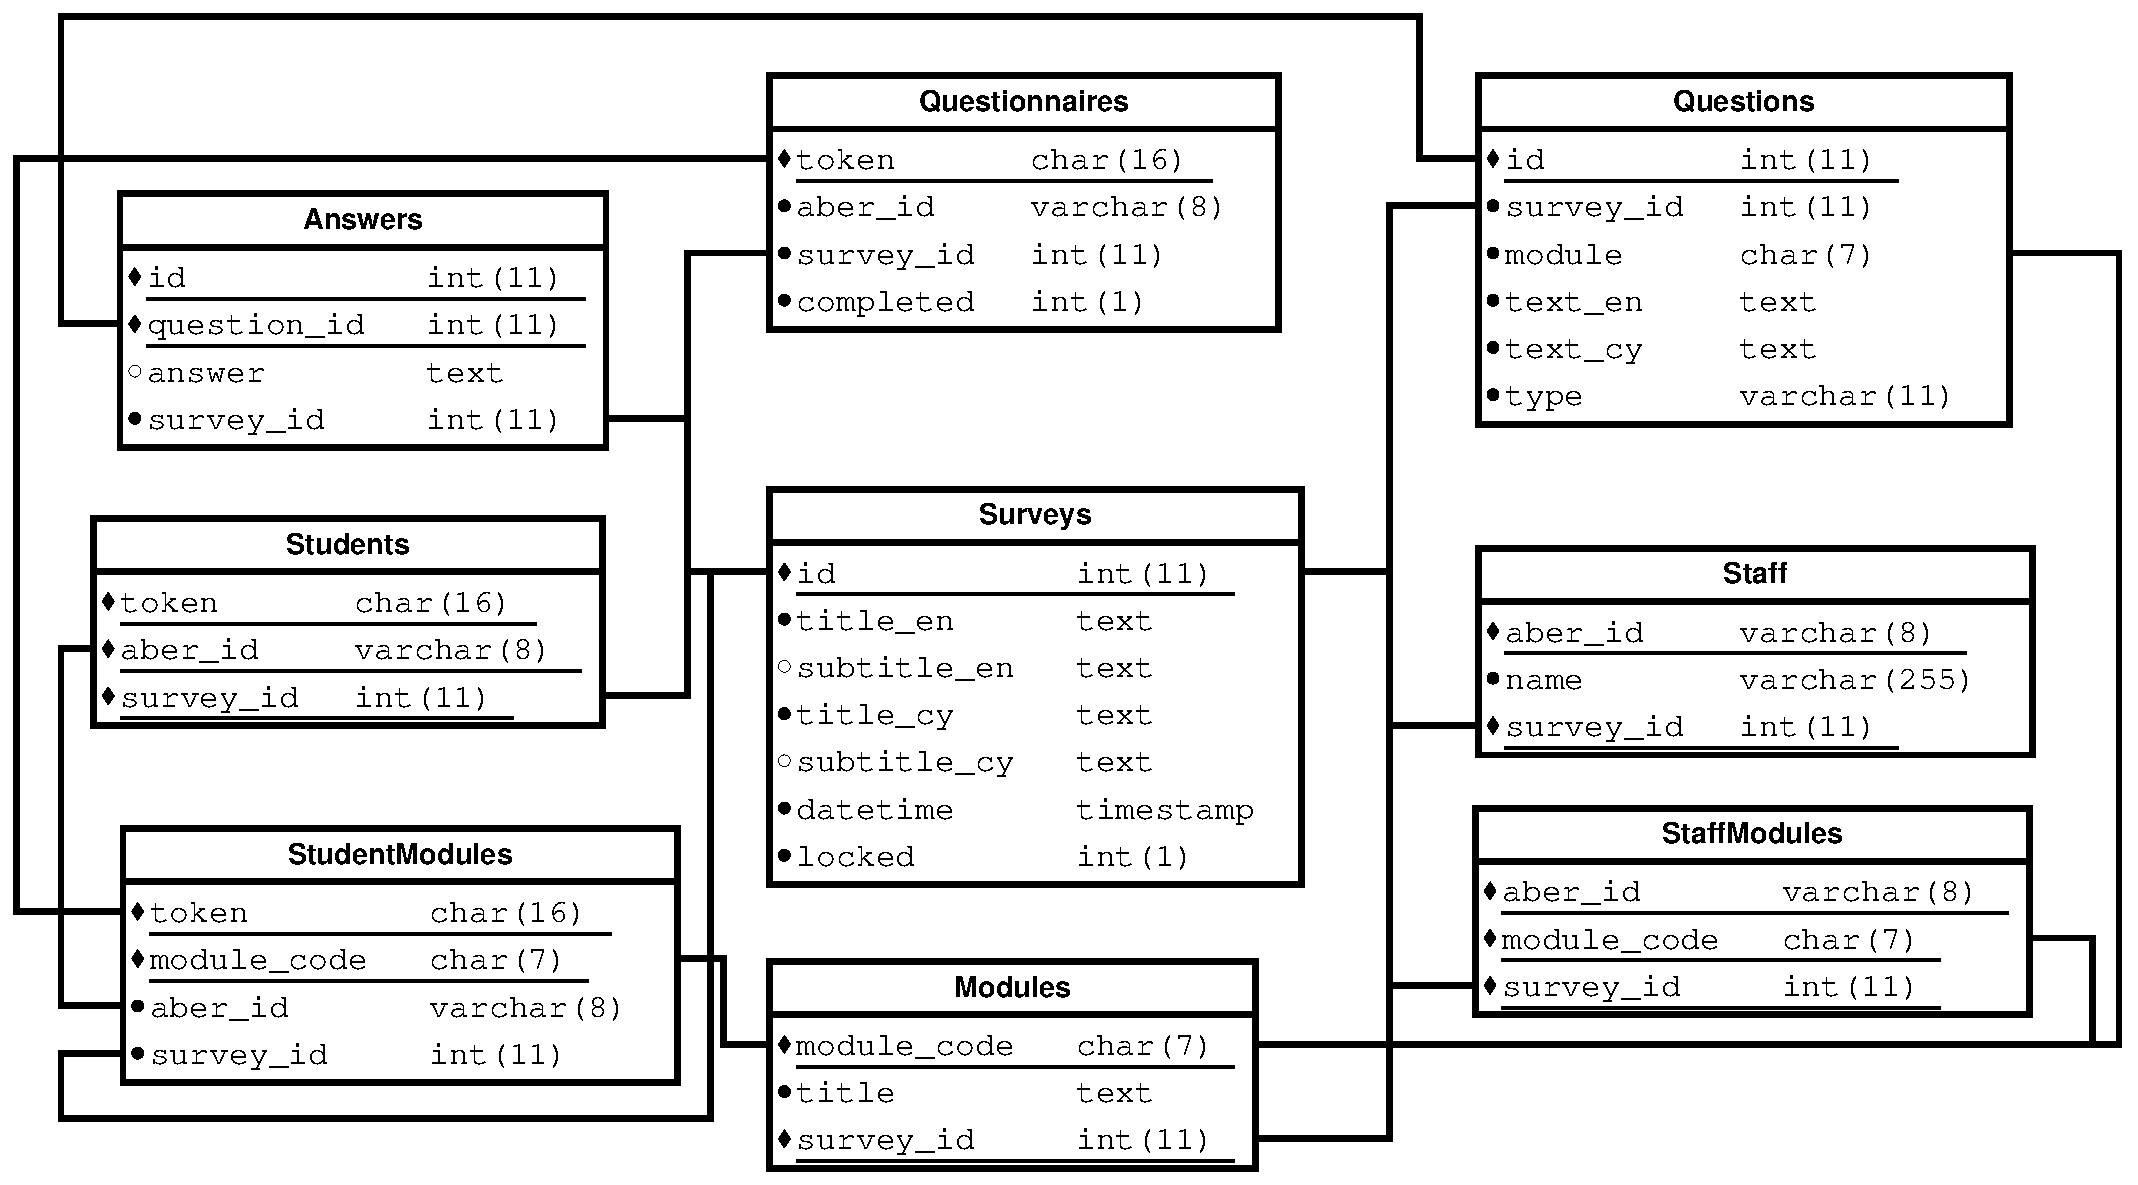
\includegraphics[width=1.33\textwidth]{schema}
		\caption{\ac{AWESOME} database schema design.}
		\label{fig:schema}
	\end{figure}
	
	\section{User Interface}
	
	The user interface was fairly good on the questionnaire-side in the prototype, so a lot of elements were re-used in that, with a few minor changes.
	
	\autoref{fig:questionnaire-comparison} shows a comparison between the prototype version and the submitted version of \ac{AWESOME}.
	
	\begin{figure}[H]
		\includegraphics[width=\textwidth]{screens/prototype-questionnaire}
		\includegraphics[width=\textwidth]{screens/final-questionnaire}
		\caption{A comparison of questionnaire pages between the prototype version and the submitted version of \acs{AWESOME}}
		\label{fig:questionnaire-comparison}
	\end{figure}
	
	The admin dashboard of the prototype wasn't very user friendly.
	Creating surveys, adding questions, modules, students, and staff was fairly convoluted.
	Results weren't clear to look at, and took up a lot of space per-question by pie charts, which were unnecessary given the data provided.
	
	\begin{figure}[H]
		\includegraphics[width=\textwidth]{screens/prototype-viewall}
		\includegraphics[width=\textwidth]{screens/final-viewall}
		\caption{A comparison of surveys view between the prototype version and the submitted version of \acs{AWESOME}}
		\label{fig:surveys-comparison}
	\end{figure}
	
	\begin{figure}[H]
		\includegraphics[width=\textwidth]{screens/prototype-results}
		\includegraphics[width=\textwidth]{screens/final-results}
		\caption{A comparison of results between the prototype version and the submitted version of \acs{AWESOME}}
		\label{fig:results-comparison}
	\end{figure}
	
	\begin{figure}[H]
		\includegraphics[width=\textwidth]{screens/prototype-single}
		\includegraphics[width=\textwidth]{screens/final-questions}
		\caption{A comparison of survey view between the prototype version and the submitted version of \acs{AWESOME}}
		\label{fig:view-comparison}
	\end{figure}
	
	\begin{figure}[H]
		\includegraphics[width=\textwidth]{screens/prototype-respondents}
		\includegraphics[width=\textwidth]{screens/final-respondents}
		\caption{A comparison of respondents between the prototype version and the submitted version of \acs{AWESOME}}
		\label{fig:respondents-comparison}
	\end{figure}
	
	Additional features include a feedback form when \ac{AWESOME} is in debug mode.
	This allows users to send an email to developers, containing any text they wish, as well as automatically including user-agent and other metadata to help identify the problem.
	
	\begin{figure}[H]
		\includegraphics[width=\textwidth]{screens/final-feedbackform}
		\caption{A screenshot of the feedback form in \acs{AWESOME}}
		\label{fig:feedbackform}
	\end{figure}
	
	\chapter{Implementation}

	\section{Prerequisites}
	\label{sec:prerequisitesimp}
	
	\subsection{Third-party services}
	\label{ssec:third-party-services}
	
	\ac{AWESOME}'s development relies on the use of a few third-party services in order to make development a little easier.
	By setting up these at the very start, valuable time and effort can be saved further down the project's lifecycle.
	
	TravisCI\footnote{TravisCI Homepage: \url{http://travis-ci.com}} was the first service I set up after receiving access to the GitHub repository.
	Travis allows for completely automated running of unit test suites whenever code is committed to Git.
	This is incredibly useful when working with modular libraries like the \ac{i18n} framework.
	Travis also allows for testing across PHP versions, so I could simultaneously test PHP 5.3, 5.4, 5.5, 5.6 and hhvm (a custom PHP server).
	
	\autoref{fig:travisbuild} shows when I made a change using a function that was new to PHP 5.6 that I wouldn't have noticed without Travis until a later date, as my development environment was running PHP 5.6.
	
	Travis proved invaluable at times, although I could have made much better use of it by unit testing much more of \ac{AWESOME}, especially the \ac{MVC} framework.
	
	Another third party service used was GitHub Pages.
	Pages allows you to publish a website from a GitHub repository branch, which is very ideal for this situation, as all code and host settings are tied to the \ac{AWESOME} Git repository which will be easy to hand over to other developers.
	
	The Pages website can be visited at \url{http://bbrks.github.io/AWESOME}.
	It is currently running Keiron's website which displays information about the prototype version of \ac{AWESOME}.
	
	\begin{figure}[H]
		\centering \includegraphics[width=\textwidth]{screens/travis-build}
		\caption{A screenshot of a single build in TravisCI}
		\label{fig:travisbuild}
	\end{figure}
	
	\begin{figure}[H]
		\centering \includegraphics[width=\textwidth]{screens/travis-build-history}
		\caption{A screenshot of build history in TravisCI}
		\label{fig:travisbuildhistory}
	\end{figure}
	
	
	\subsection{Open Source License}
	\label{ssec:license}
	
	The prototype version of \ac{AWESOME} was originally under the open-source MIT license\cite{mitlicense} when branched and my work began.
	Some time after this point, the license on the original was changed to the GNU Affero General Public License, Version 3\cite{gplv3afferolicense}, however as I had branched the prototype version as it stood under the MIT license, the largely-rewritten version of \ac{AWESOME} is also licensed under the MIT license and does not touch any code licensed under the GPL v3 Affero license and so I am not restricted to using a GPL-based license.
	
	\ac{AWESOME} uses an open source, third party library for handling mail via SMTP called PHPMailer\cite{phpmailer} which is licensed under the LGPL v2 license.
	This license permits me to release \ac{AWESOME} under the MIT license without any license impositions that GPL would.
	
	Bootstrap, jQuery and jQuery StickyTabs plugin are used in the project, all of which are released under the MIT license, which again, has no restrictions on what license I have to use.
	
	\subsection{Development Environment}
	\label{ssec:devenvironment}
	
	I developed locally on my personal laptop, a MacBook Pro Retina, which ran OS X 10.10.1 at the start of this project, and now 10.10.3 at the end.
	The web server is running from Apache with PHP 5.6 via Homebrew, although later downgraded to match the PHP environment on the \ac{AU} server.
	
	Code was written in SublimeText, and most of the browser testing took place under Google Chrome and on a Nexus 5 phone.
	Git was handled through the command line, as was the compilation of \LaTeX.
	SequelPro\footnote{SequelPro Homepage: \url{http://www.sequelpro.com}} was used to connect to databases both locally and remotely.
	
	Sketch\footnote{Sketch Homepage: \url{http://bohemiancoding.com/sketch}} was used for the creation of logos and other graphics used in \ac{AWESOME}, and Dia\footnote{Dia Homepage: \url{http://dia-installer.de}} was used to create the \ac{UML} diagrams and database schema design in this report.
	
	\section{Security Audit and Code Review}
	\label{sec:securityauditimp}
	
	The security audit of \ac{AWESOME} was one of my first tasks on this project and it uncovered some issues.
	First of all, the admin login accepted any credentials, and secondly, the mysqli functions used to connect to the database are no longer recommended to be used.
	Instead, \ac{PDO} should be used to connect to databases, as this provides much better security through prepared statements, preventing SQL injection attacks.
	
	The prototype was also written in a completely procedural style, with if statements for each bit of \acl{i18n} spread throughout the codebase.
	Rewriting to use \ac{OOP} practices as well as a design pattern would kill several birds with one stone, as I could also implement \ac{PDO} and proper \ac{i18n} whilst I was at it.
	
	\section{\acl{MVC} Framework}
	\label{sec:mvcframeworkimp}
	
	The \acl{MVC} framework was fairly straight forward to code at first, especially following the tutorial mentioned previously\cite{php-mvc-tutorial}.
	However I soon ran into limitations of the framework, and the time to code in additional features ate away at the time I needed to produce a working survey tool.
	
	In the end, \ac{AU} server limitations forced me to throw away most of the functionality in the \ac{MVC} framework.
	
	\section{\acl{i18n} Framework}
	\label{sec:i18nframeworkimp}
	
	The \ac{i18n} system is small but very useful, albeit not as flexible or powerful as a mature \ac{i18n} framework.
	It has no ability to pluralise strings, nor does it offer any variable substitution like some frameworks might be expected to do.
	This lack of complexity, I think makes it better for non-technical people to provide language translations though, as everything is read in through simple JSON files.
	
	
	
	\section{Deploying to an \ac{AU} server}
	\label{sec:auserverimp}
	
	Getting \ac{AWESOME} running on a server at \ac{AU} took much longer than anticipated for a few reasons.
	Firstly, the PHP version was 5.3, which was attempted to be upgraded to 5.6, but it didn't work out, so I had to change some code to ensure it was 5.3 compatible.
	Secondly, I didn't have any direct access to the server, so any change that was made had to be zipped, sent via email to Sandy, and then he would upload the files for me, provided it was between 9am and 5pm on a weekday.
	Another issue was that the database would not connect, even though it was configured correctly.
	This was solved by Sandy adding a wildcard rule to the database hostname limit, which enabled connection from any machine.
	This poor access coupled with troubleshooting issues regarding PHP version and database connections issues were a serious hinderance.
	
	Once these issues were resolved, \ac{AWESOME} was working on the university server okay, with one condition.
	The server I was on could only be accessed through the \ac{AU} \ac{VPN}, and so anybody who received a link to a questionnaire had to either be on the university network, or connected through the university VPN to be able to view it.
	Another issue is that HTTPS was not set up correctly, and so instead of either redirecting to HTTP, or failing a certificate check, it would not allow access to \ac{AWESOME}.
	This caused problems for people using browser plugins that forced HTTPS on websites.
	
	Because of these issues, I feel that response rates through \ac{AWESOME} are significantly lower than they would otherwise be, despite being around the same 20\% figure that Google Forms had.
	
	I feel that once server access is properly fixed, response rates could be 50\% or even higher, which is a significant improvement upon previous online module evaluation methods.
	\chapter{Testing}
	
	\section{Automated Testing}
	
	For this project, a \ac{CI} platform was chosen to be used in order to facilitate automated unit tests.
	By using \ac{CI} ensured that every time code was committed with unit tests, the suite was ran and results were instantly available.
	Any test failures resulted in a notification email being sent to identify when and where a problem had occurred.
	
	After seeing fellow classmates use TravisCI\footnote{TravisCI Homepage: \url{http://travis-ci.com}} on previous projects, and reviewing the features it provides, I decided to utilise it in this project.
	Travis offered testing across multiple PHP versions, which proved helpful when trying to provision a server on the university network.
	
	This was indispensable mid-way through the project, when functionality in the \ac{i18n} framework needed to be changed and tests started to fail.
	I wouldn't have noticed any errors when manually testing, but the unit tests brought up edge cases which were then dealt with.
	
	\section{User Testing}
	
	User testing was carried out by creating a survey and entering volunteer's \ac{AU} usernames in the student \ac{CSV} data along with sample modules.
	The first real test through the \ac{AU} servers was sent to staff.
	This uncovered many issues with the setup of \ac{AWESOME} on the \ac{AU} server, which took some time to fix.
	After these issues were resolved, an end-of-semester questionnaire was sent out to the vast majority of students in the Computer Science department. From first years, to masters students.
	
	User testing revealed some useful information via the feedback form, as well as through a question in the survey which was asked about how easy \ac{AWESOME} was to use.
	
	\section{Acceptance Testing}
	
	Acceptance testing was carried out on the submitted version of \ac{AWESOME} and results in test tables can be found in Appendix \autoref{app:testtables} with 16/18 (89\%) of tests passing.
	More detail of the two failing tests can be found in the appendix entry.

	\chapter{Evaluation}
	
	\section{Process}
	
	\section{Development Environment}
	
	\section{Project Stages}
	
	\section{Blog}
	
	\section{Degree}
	
	\section{Upper Management}
	
	\section{Time Management}
	
	\section{Future Scope}
	

	\bibliographystyle{ieeetr}
	\bibliography{bibliography}

	\begin{appendices}

	\chapter{Appendix 1}
		Lorem ipsum\ldots
	
\end{appendices}


\end{document}
